\documentclass[10pt]{beamer}

\usetheme{metropolis}
%\metroset{background=dark}
%\usepackage{appendixnumberbeamer}
\usepackage{tikz}
\usepackage{fontawesome}
\usetikzlibrary{positioning}
\definecolor{cobaltBlue}{HTML}{38ACEC}
%\setbeamercolor{alerted text}{fg=cobaltBlue}
\usepackage{booktabs}
\usepackage[scale=2]{ccicons}

\usepackage{pgfplots}
\usepgfplotslibrary{dateplot}

\usepackage{xspace}

\newcommand{\lift}{\textsc{lift}\space}

%\setbeamercolor*{structure}{bg=black,fg=white}


\title{Lift Tutorial: Applications}
\date{}
%\author{\textbf{Larisa Stoltzfus}}
%\institute{\textbf{PPar Cohort 2015}}

\begin{document}

\begin{frame}[plain,noframenumbering]
\maketitle
\end{frame}

\section{Writing an Application}

\begin{frame}
\frametitle{General Steps}
\begin{itemize}
    \item Determine input parameters 
    \item Initialise input data 
            \begin{itemize}
                \item If testing, initialise comparison data 
            \end{itemize}
    \item Craft or translate the algorithm of interest 
    \item Determine what memory to use running the resulting kernel 
    \item Create an OpenCL kernel from your algorithm 
\end{itemize}
\end{frame}

\begin{frame}
\frametitle{Data Input to Lift Algorithms}
\begin{itemize}
    \item Lift takes in arrays as input parameters
            \begin{itemize}
                \item Single values can be passed in in array form or used as global values
            \end{itemize}
\begin{block}{}
    \begin{center}
    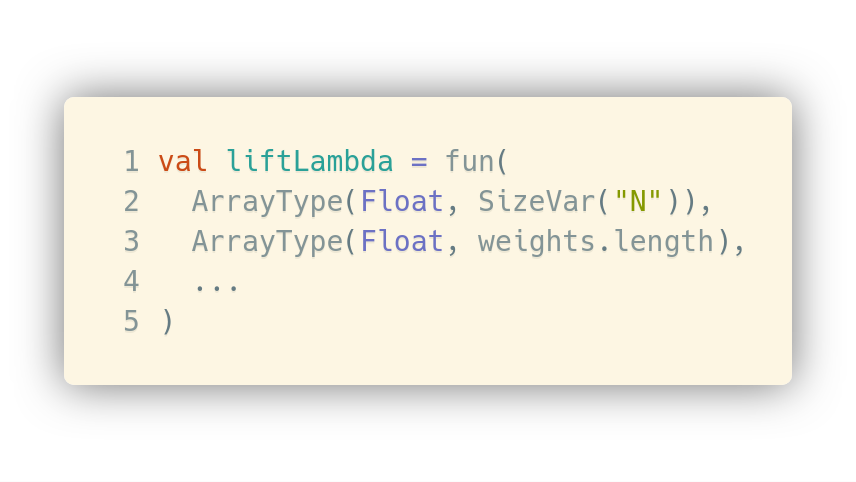
\includegraphics[width=.5\textwidth]{../images/inputData.png}
    \end{center}
\end{block}
    \item Single entry point for arrays into functions  
            \begin{itemize}
                \item Multiple arrays can be zipped together (but must be the same size!) 
            \end{itemize}
            \vspace{-.4cm}
\begin{block}{}
    \begin{center}
    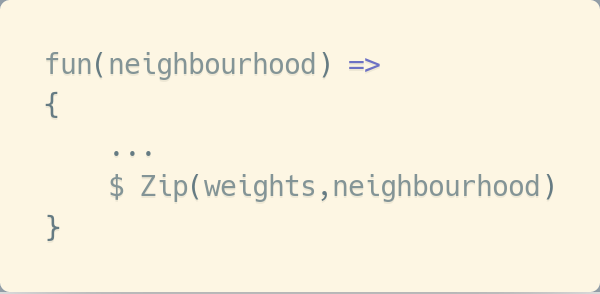
\includegraphics[width=.5\textwidth]{../images/zippedData.png}
    \end{center}
\end{block}
\end{itemize}
\end{frame}

\begin{frame}
\frametitle{Initialising Data in Scala}
\begin{itemize}
    \item Create arrays of data to pass into Lift algorithms in Scala 
        \vspace{-.5cm}
\begin{block}{}
    \begin{center}
         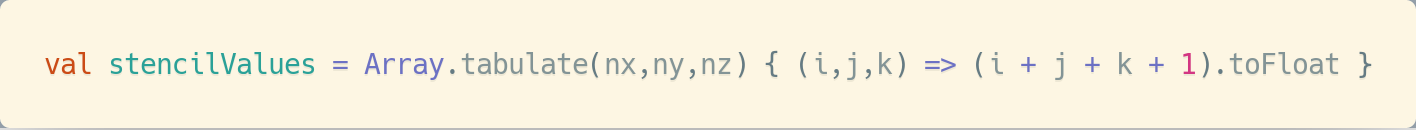
\includegraphics[width=.85\textwidth]{../images/scalaArrays.png}
    \end{center}
\end{block}
    \item Our examples are all in unit tests, which include data to compare against - often from the same algorithm in Scala 
        \vspace{-.5cm}
    \begin{block}{}
        \begin{center}
            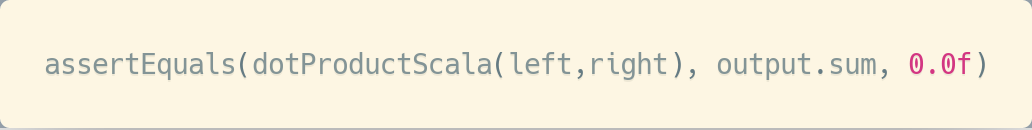
\includegraphics[width=.85\textwidth]{../images/unitTestData.png}
        \end{center}
    \end{block}
\end{itemize}
\end{frame}

\begin{frame}
\frametitle{Developing an Algorithm}
The goal is not for Lift to be programmed in directly.\\
\vspace{.1cm}
However, functionality for new types of algorithms must be added in and tested. In doing so, there are a few things to keep in mind: 
\begin{itemize}
    \item Lift allows multiple inputs, but there is only one data entry point to the main algorithm (can contain tuples)
    \item The algorithm itself must eventually map values back to global memory
    \item The result will be returned in a single array (however, this array can also contain tuples)
\end{itemize}
\end{frame}

\begin{frame}
\frametitle{Simple Example: 1D Jacobi Stencil}
\begin{block}{}
    \begin{center}
    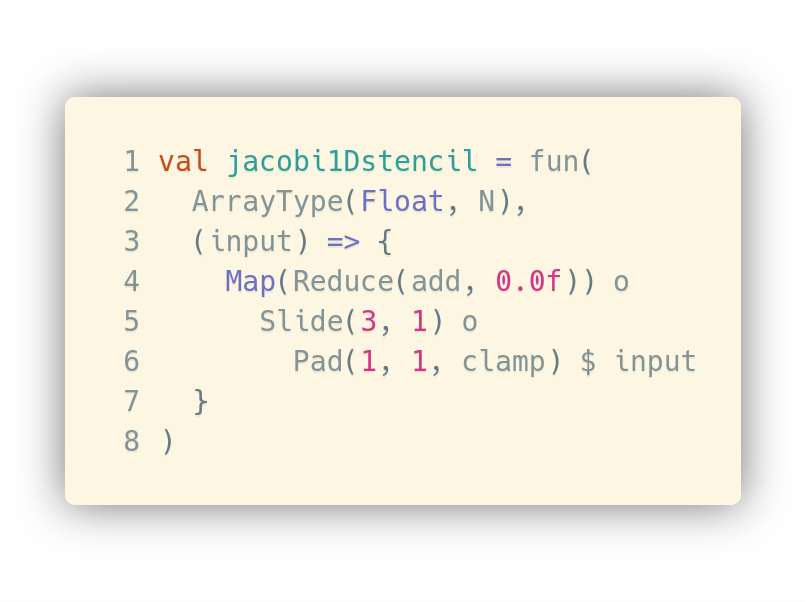
\includegraphics[width=.5\textwidth]{../images/jacobi1Dstencil.png}
    \end{center}
\end{block}
\end{frame}

\begin{frame}
\frametitle{Memory Options}
\begin{itemize}
    \item There are a range of different OpenCL memories that can be targeted in an algorithm 
        \begin{itemize}
            \item MapGlb - use global memory
            \item MapWrg - use workgroup memory
            \item MapLcl - use local memory
        \end{itemize}
    \item Can parallelise up to 3 dimensions in OpenCL 
        \vspace{-.5cm}
    \begin{block}{}
        \begin{center}
            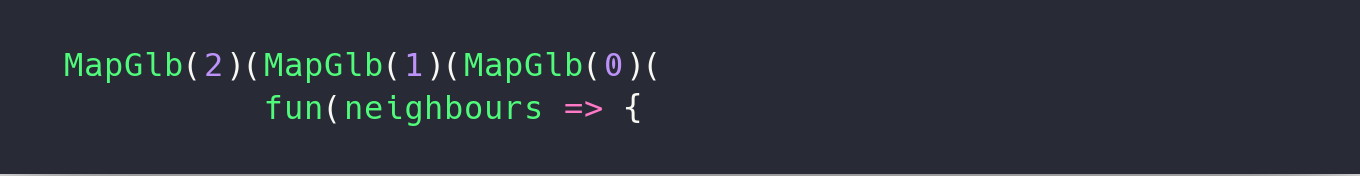
\includegraphics[width=.85\textwidth]{../images/mapMapMap.png}
        \end{center}
    \end{block}
\end{itemize}

%        \begin{center}
%            \begin{columns}
%    \begin{column}{.3\textwidth}
%        \begin{block}{}
%            %\hspace{-.03cm}
%            \includegraphics[width=3.8cm, height=2.5cm]{../images/soundwaves.png}
%        \end{block}
%        \end{column}
%        \begin{column}{.3\textwidth}
%            \LARGE\begin{equation*}\frac{\partial^2 \Psi}{\partial t^2} = c^2\nabla^2 \Psi\end{equation*}
%           % \begin{block}{}
%           %     % Your text here
%           % \end{block}
%        \end{column}
%    \begin{column}{.3\textwidth}
%        {
%            \setbeamercolor{block body}{bg=white}
%        \begin{block}{}
%            %\hspace{-.03cm}
%            \includegraphics[width=.95\textwidth]{../images/stencil.pdf}
%        \end{block}
%    }
%        \end{column}
%    \end{columns}
%\end{center}
\end{frame}


\begin{frame}
\frametitle{Creating an OpenCL kernel}
\begin{itemize}
    \item To compile your Lift kernel to OpenCL, run [opencl.executor]Compile(\textit{<kernel>}) 
        \begin{itemize}
                \item This kernel can then be saved as a string or file
        \end{itemize}
        \vspace{-.7cm}
        \begin{block}{}
        \begin{center}
            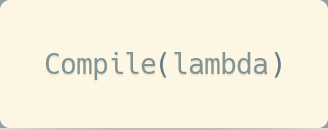
\includegraphics[width=.5\textwidth]{../images/simpleCompile.png}
        \end{center}
        \end{block}
    \item To execute the kernel straight away (compiling will happen behind the scenes), run [opencl.executor]Execute(\textit{<options>})[Array[\textit{type}](\textit{lambda}, \textit{..inputs..}) 
    \begin{block}{}
        \begin{center}
            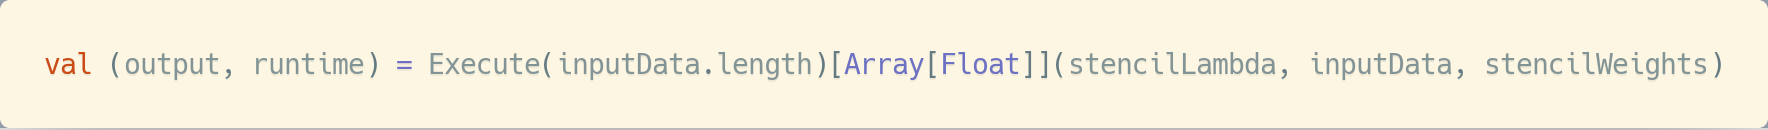
\includegraphics[width=\textwidth]{../images/execute.png}
        \end{center}
    \end{block}
\end{itemize}
\end{frame}


\section{Detailed Example: Matrix-Matrix Multiplication }

\begin{frame}
\frametitle{Matrix-Matrix Multiplication Overview}
\vspace{.2cm}
\begin{itemize}
    \item Widely used algorithm in mathematics, physics, engineering, etc
    \item Range of possible optimisations can be used, the performance of which varies across architectures
    \item Lift makes it easy to test these optimisations out without having to rewrite the original code 

\end{itemize}
\vspace{-1.2cm}
\end{frame}

\begin{frame}{Matrix-Matrix Multiplication Example Code}
        \begin{block}{}
        \begin{center}
            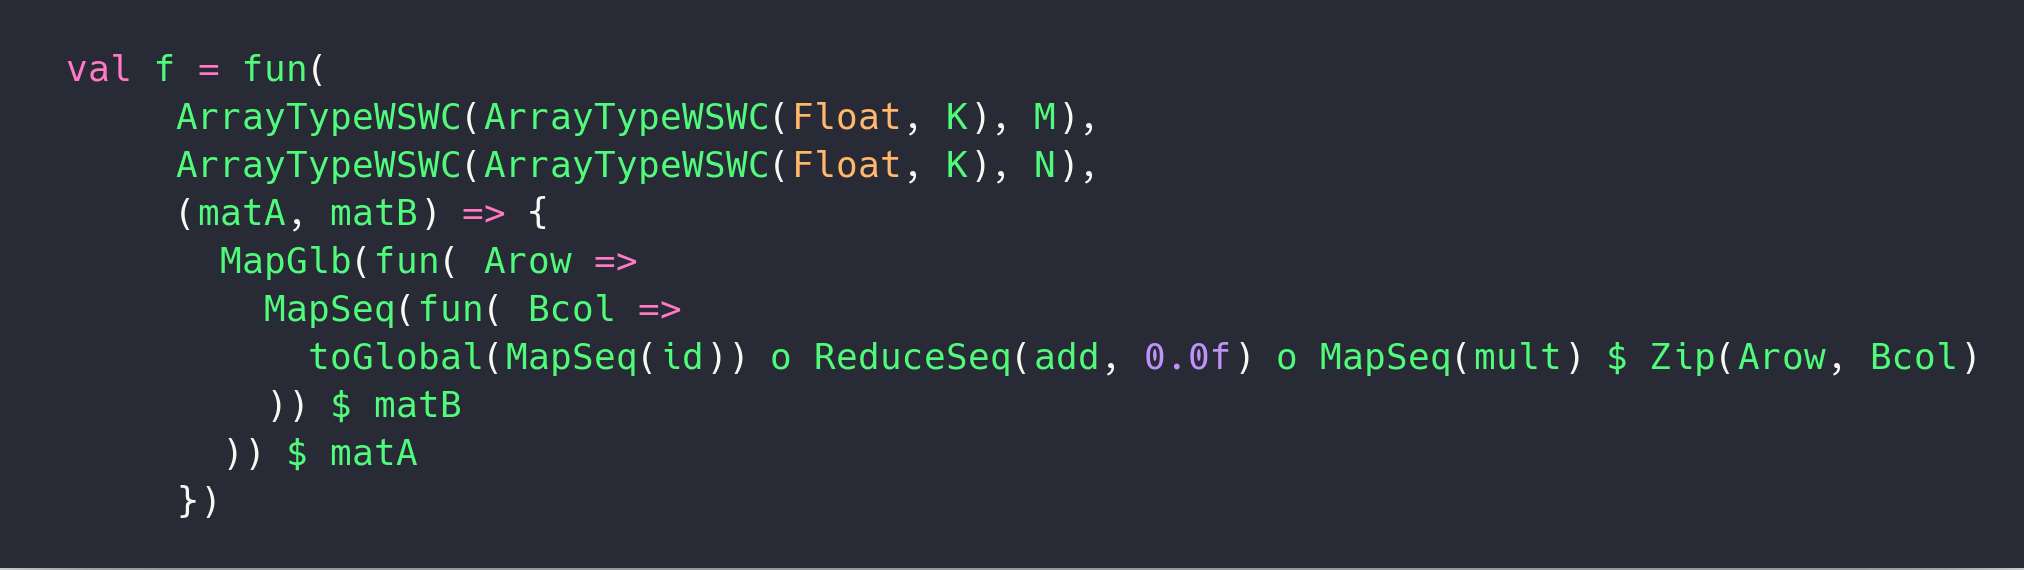
\includegraphics[width=\textwidth]{../images/matrixMatrix.png}
        \end{center}
        \end{block}
\end{frame}

\begin{frame}{Matrix-Matrix Multiplication Using Rewrites}
        \begin{block}{}
        \begin{center}
            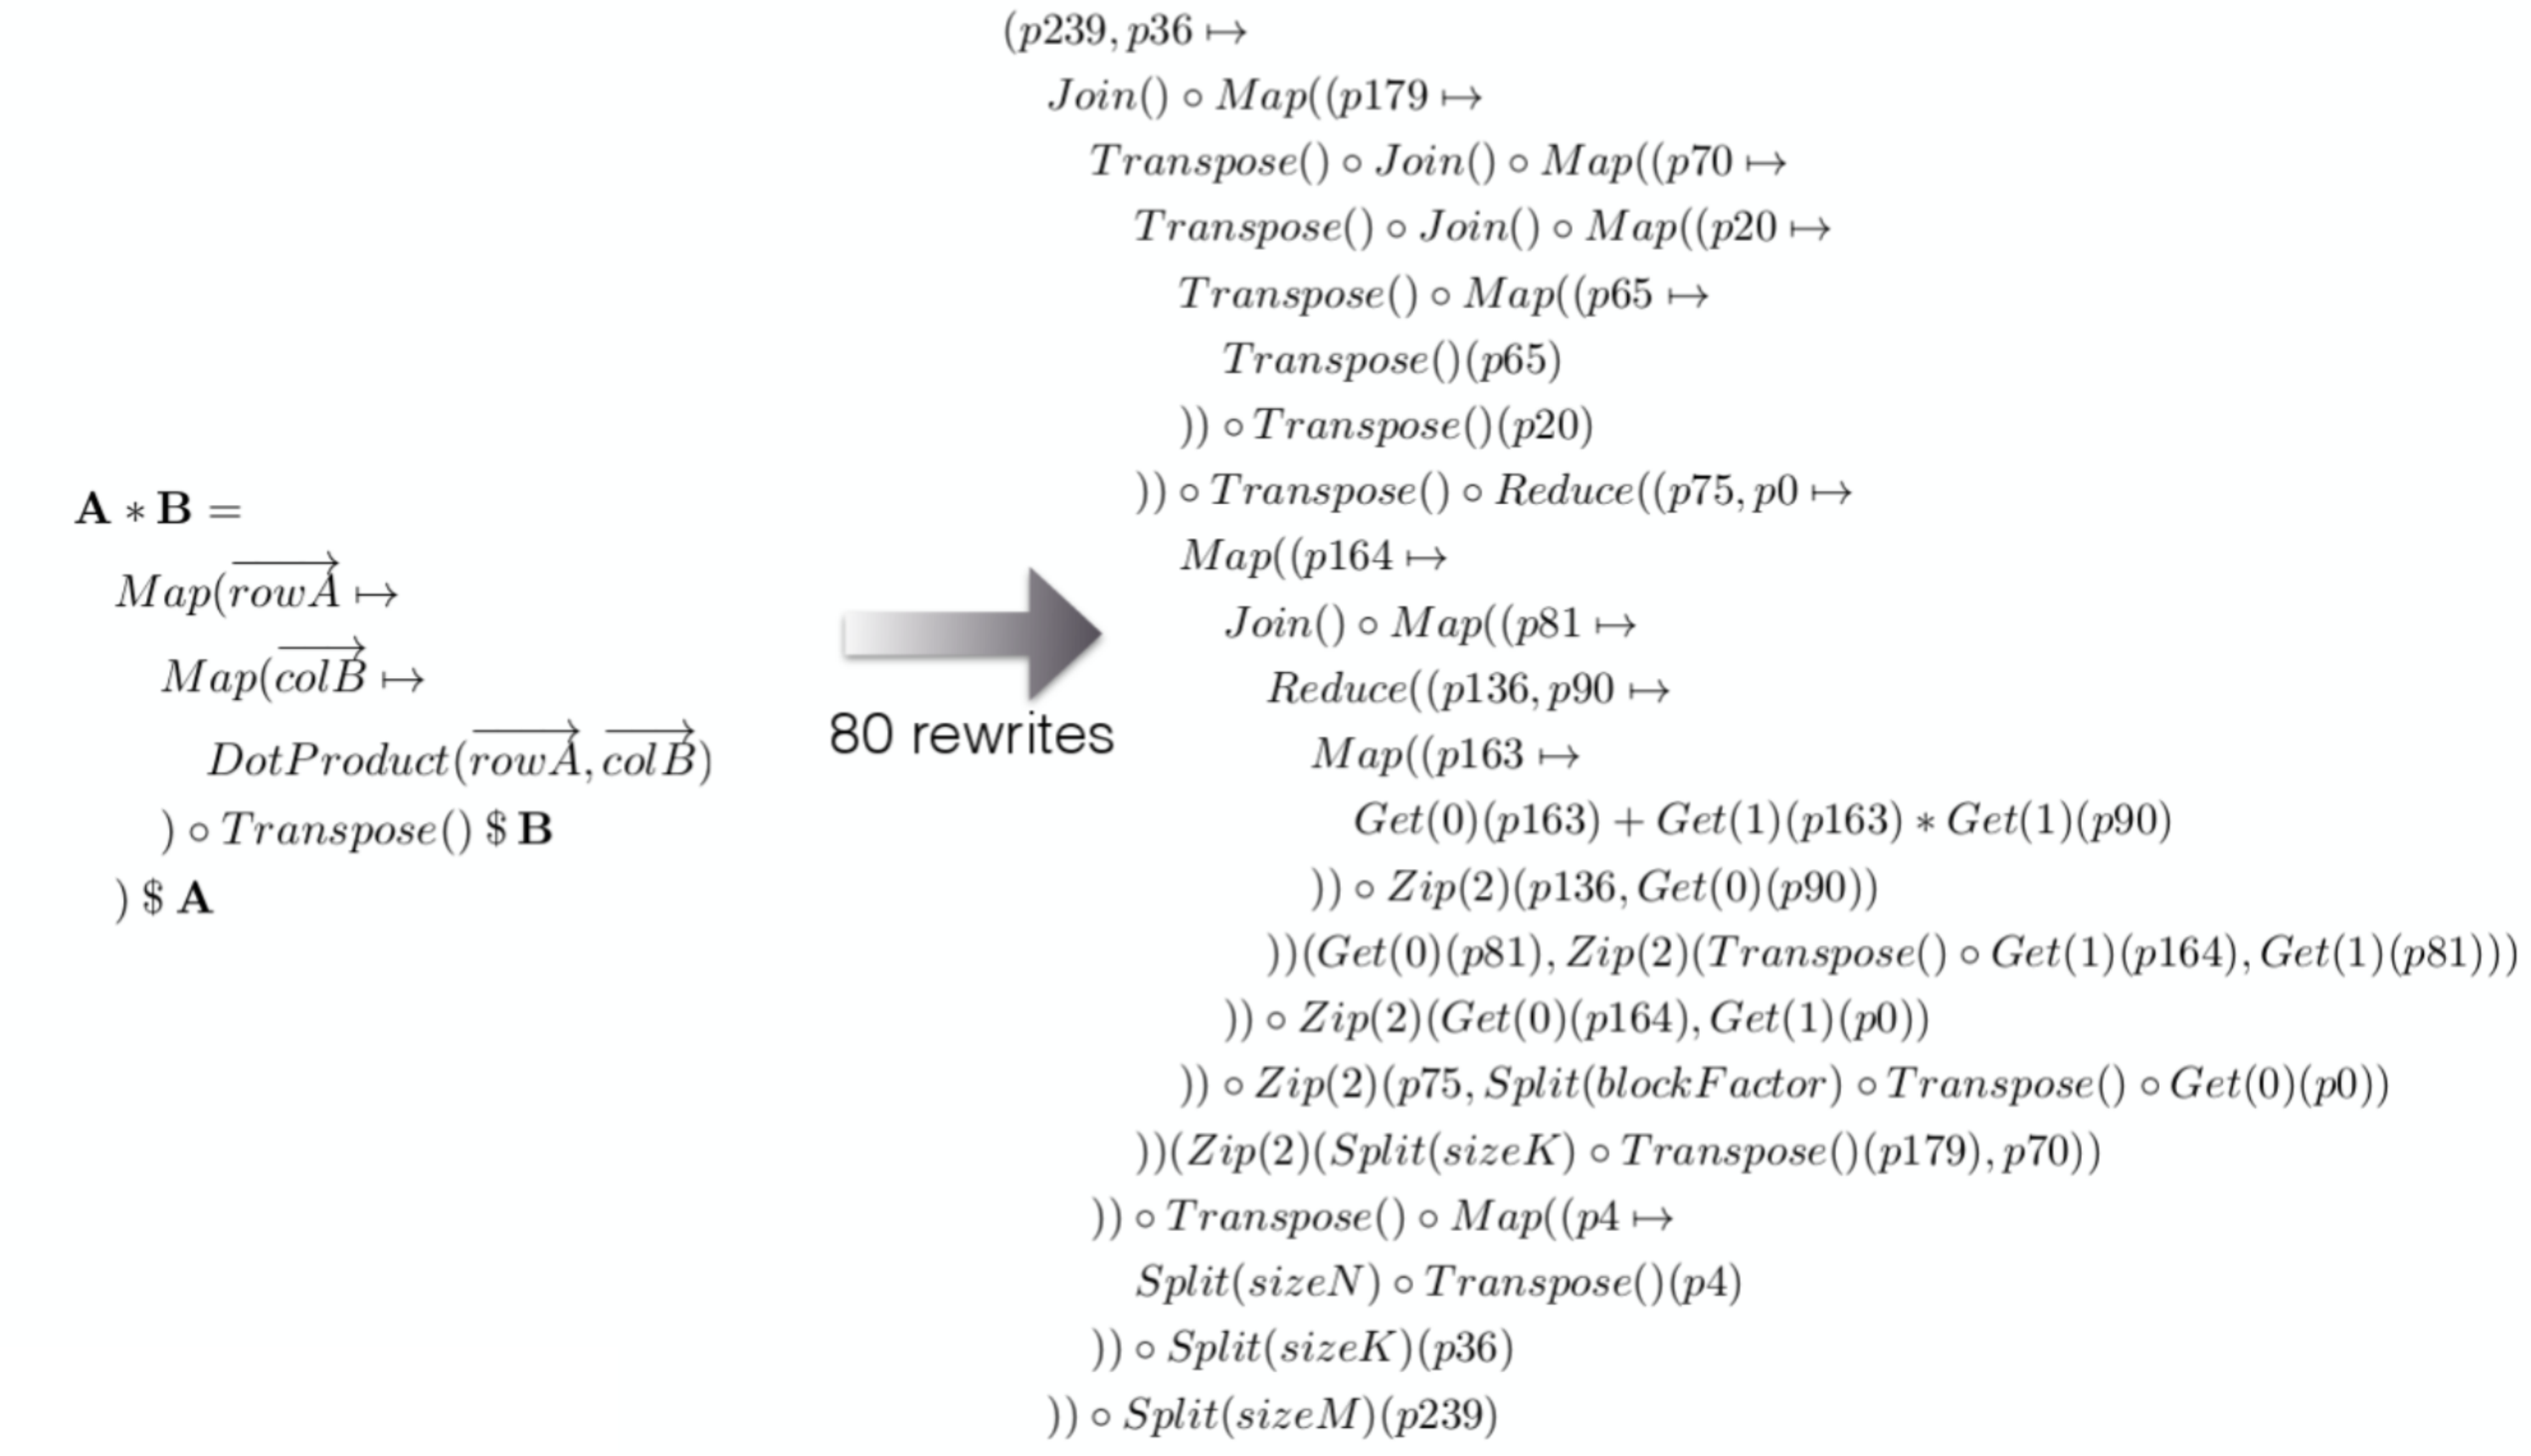
\includegraphics[width=\textwidth]{../images/matrixRewrites.pdf}
        \end{center}
        \end{block}
\end{frame}


\section{Detailed Example: Convolutional Neural Network }

\begin{frame}
\frametitle{Convolutional Neural Network -- Overview}
\vspace{-.5cm}
    \begin{block}{}
        \begin{center}
            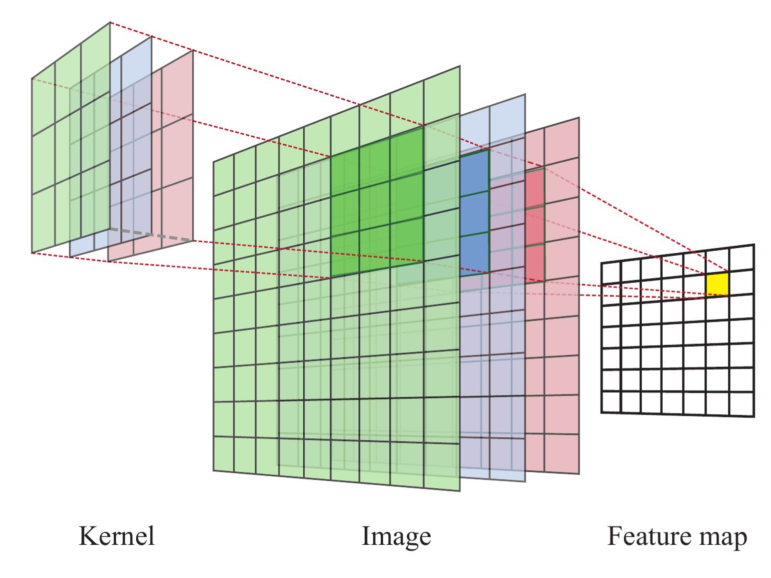
\includegraphics[width=0.8\textwidth]{../images/conv.pdf}
        \end{center}
    \end{block}
\vspace{-1.2cm}
\end{frame}

\begin{frame}{Convolutional Neural Network -- Parallel Implementation}
\vspace{-1.5cm}
    \begin{block}{}
        \begin{center}
            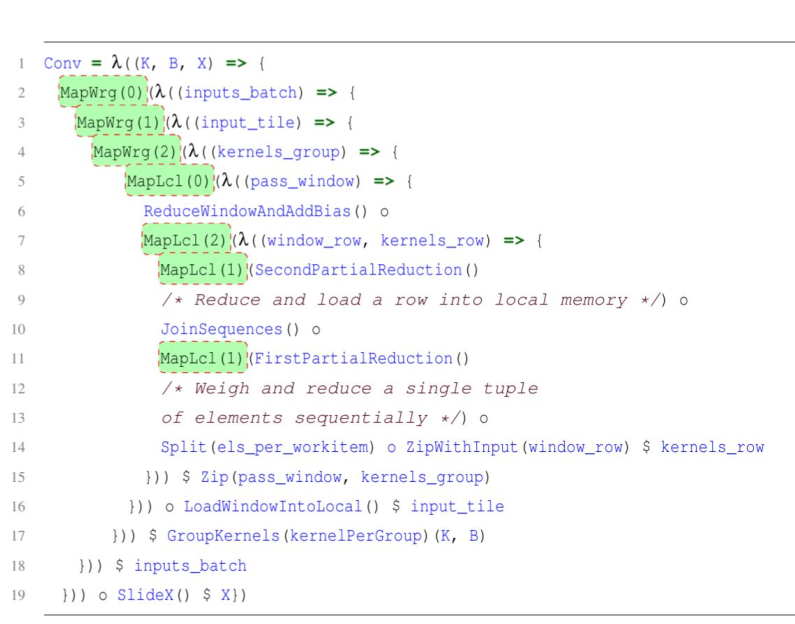
\includegraphics[width=0.8\textwidth]{../images/conv_expr_par.pdf}
        \end{center}
    \end{block}
\vspace{-1.2cm}
\end{frame}

\begin{frame}{Convolutional Neural Network -- OpenCL ND space}
\vspace{-1.5cm}
    \begin{block}{}
        \begin{center}
            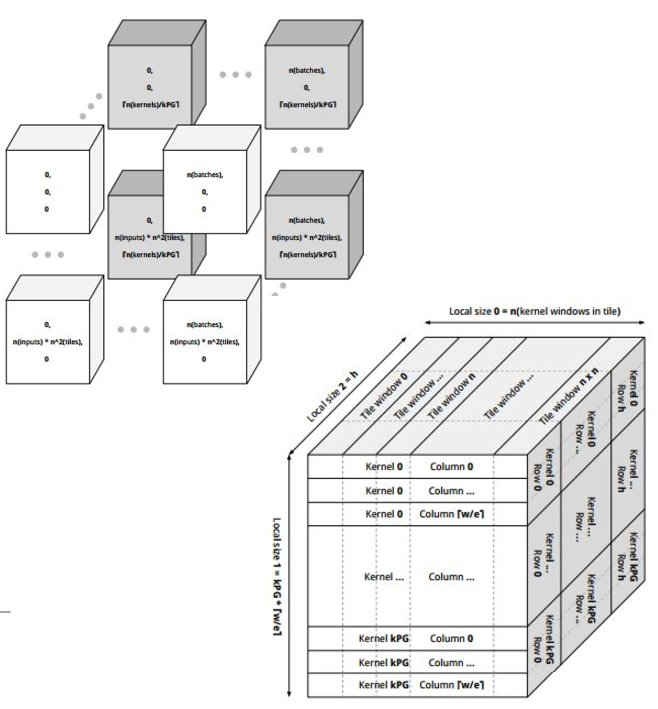
\includegraphics[width=0.7\textwidth]{../images/conv_nd.pdf}
        \end{center}
    \end{block}
\vspace{-1.2cm}
\end{frame}

\section{Detailed Example: Acoustics Simulation }

\begin{frame}
\frametitle{Acoustics Simulation Overview}
\vspace{.2cm}
\begin{itemize}
    \item Partial Differential Equations can be discritised into stencils to model physical simulations like 3D wave models 
    \item A simple acoustics simulation shows how this can be done in Lift 
\end{itemize}
\vspace{-1.2cm}
\end{frame}

\begin{frame}{Acoustics Simulation Example Code}
        \begin{block}{}
        \begin{center}
            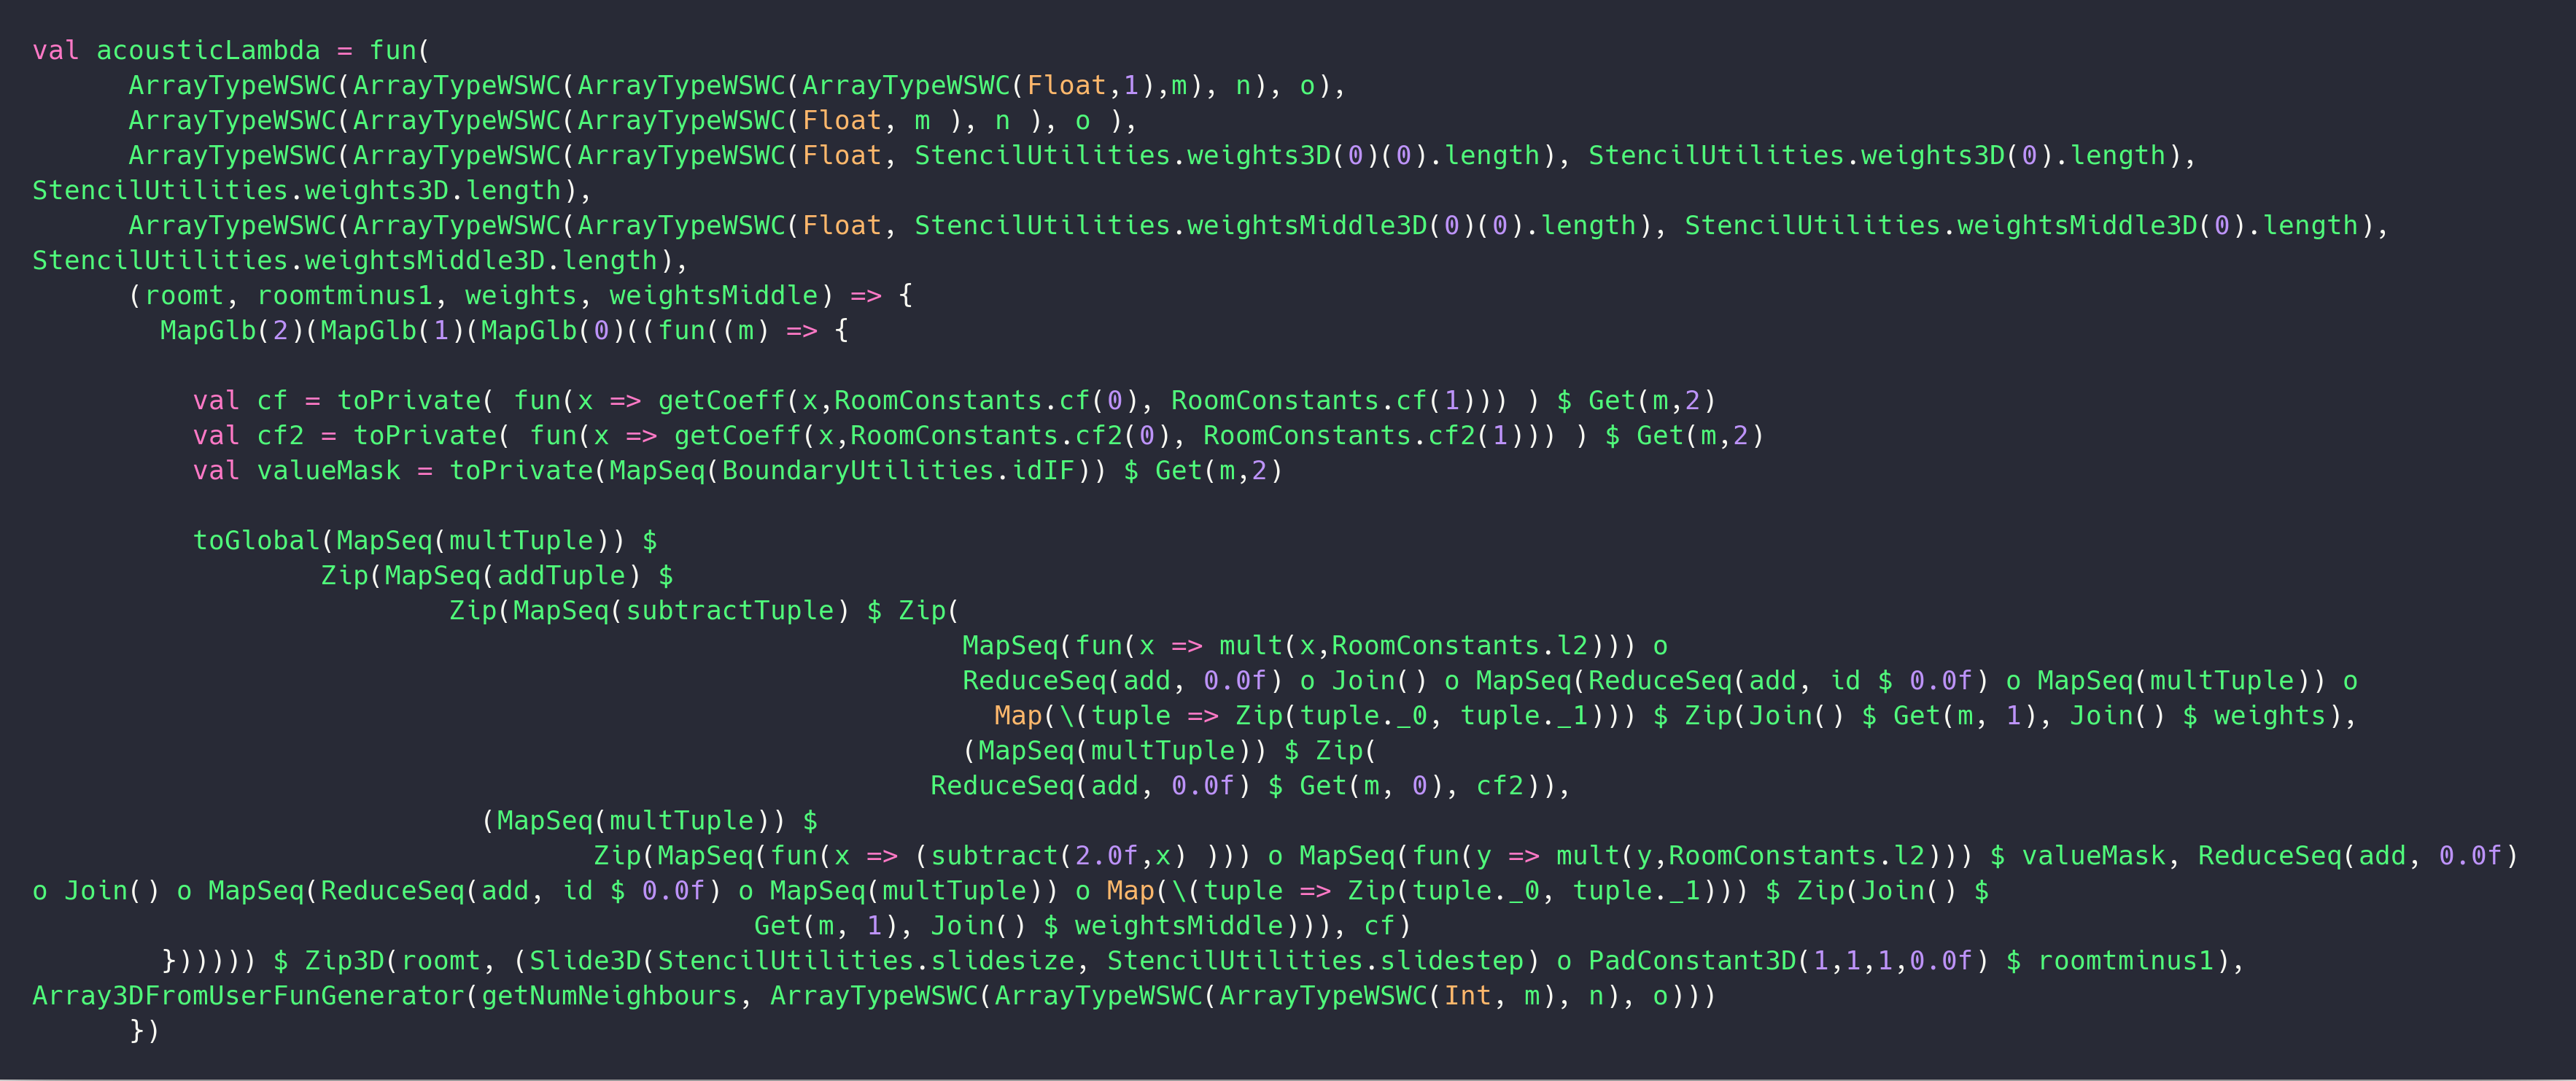
\includegraphics[width=\textwidth]{../images/acousticLambda.png}
        \end{center}
        \end{block}
\end{frame}

\appendix

\end{document}
